In \iref{ch:your-first-model} you downloaded the \concept{\US\ Installer}. This installer put the \US\ application on your computer, together with a selection of box scripts. What was not included in the installer was the \concept{\protect\US\ source code}.

You need the \US\ source code to code your own boxes in \CPP. First you download the source code, then you extend it with your own coding. Source code is turned into a working application through the process known as \concept{build}. When you have built \US\ yourself, the \US\ application will exist in two incarnations on your computer: (1) the one you got with the installer and (2) the one you built. However, they will share the same \inputfolderexplained\ folder, so they will work with the very same input files (\eg\ box scripts).

\section{First time build}
Here are, in short, the steps to go through for you first build of \US. A more detailed walk-through of the process is given in \iref{ch:workflow}. Before you build, make sure you have installed Qt Creator (\iref{ch:install-qt}) and Boost (\iref{ch:install-boost}).

\begin{enumerate}
\item Download the latest version of \US\ source code from \url{https://github.com/NielsHolst/UniSim2/releases}. Click the \gui{zip} button to download.
\item Unzip the downloaded file. Put it as a sub-folder inside your \devhomefolderexplained\ folder. See also \iref{fig:unisim-versions}.
\item Launch Qt Creator. Choose \gui{Open File or Project} and open the \filename{UniSim2.pro} project file found in the \filename{src} sub-folder of the source code folder.
\item Qt Creator will sense that it never opened this project file before and will ask, if it should configure the project. Push the \gui{Configure Project} button (\iref{fig:build-us-1}).

\begin{figure} [h]
\centering
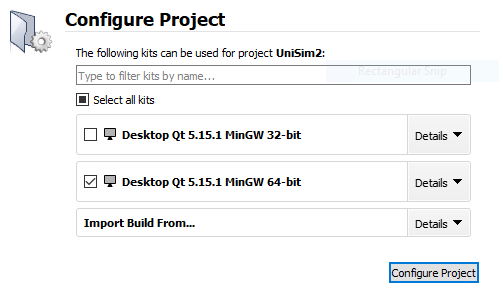
\includegraphics[width=\textwidth]{graphics/build-us-1}
\caption{First time Qt Creator opens a project, it will ask permission to configure the project.}
\label{fig:build-us-1}
\end{figure}

\item Wait while Qt Creator configures the project. The build bar in the lower right corner will show green when it's done.
\item Under Mac OS X, Qt Creator will write some files to the \filename{\mytilde/lib} folder. Make sure that this folder is writable, or else the next step will fail.
\item  In the \gui{Build} menu choose \gui{Build project "UniSim2"}.
\item Wait while Qt Creator builds the project. This will take a few minutes. You might get some warnings showing up in Qt Creator during the build. These you can ignore. The important message is the build bar turning green. Then the build has finished successfully.
\item Run \US\ by pushing the green triangle (bottom left).
\item For more details, study \iref{ch:workflow}.
\end{enumerate} 